\section[Introduzione all'uso dell'informazione di posizione]{Introduzione all'uso dell'informazione di \\posizione}
La posizione ci indica dove si trova un dispositivo in un ambiente di riferimento che può essere nel mondo, in un edificio, ecc. 
\\ Possiamo avere 2 dimensioni, dove la posizione è considerata rispetto ad un piano, oppure 3 dimensioni, dove la posizione è considerata rispetto ad un piano ed un'altezza.
Possiamo rappresentare la posizione attraverso la:
\begin{itemize}
    \item rappresentazione geografica: la posizione nel mondo 
    \item rappresentazione in coordinate locali: la posizione ad es. su una mappa 
    \item rappresentazione semantica: es. indirizzo
\end{itemize}

Nella rappresentazione geografica ci sono due sistemi di riferimento: 
\begin{itemize}
    \item latitudine: viene preso come punto di riferimento l'equatore 
    \item longitudine: viene preso come riferimento il meridiano di Greenwich 
\end{itemize}

L’informazione di posizione non riporta il tempo, ma l'informazione temporale è fondamentale da associare alla posizione in molti contesti, ad esempio se vogliamo descrivere una traiettoria, cioè una lista di elementi $<$timestamp, position$>$. 

Il calcolo della posizione (e del tempo) non è esatto. 
In termini matematici potremmo definire una funzione, di distribuzione di probabilità, che associa ad ogni punto dello spazio la probabilità che il device si trovi lì. 
In termini pratici, si modella un'area dove probabilmente si trova il device. 
Questa approssimazione però non ci dice dove si trova il device all'interno dell'area. 

\subsection{Accuratezza e precisione}
Una delle caratteristiche più rilevante di un sistema di calcolo della posizione è quanto la posizione calcolata differisce da quella reale. 
\\ Supponiamo che l’utente sia fermo e che siano date varie misurazioni della sua posizione.
Con \textit{precisione} si intende quanto le misurazioni sono vicine l'una all'altra.
Con \textit{accuratezza} si intende quanto le misurazioni siano vicine alla posizione vera.

L'errore di posizionamento viene calcolato in questo modo: indico che la posizione calcola ha un x\% di probabilità di probabilità di essere più vicina di y metri alla posizione corretta. 

Il livello di precisione non sempre è lo stesso, dipende dal tipo di applicazione e dal tipo di utente. 
Possono avere una precisione a livello di: 
\begin{itemize}
    \item regione (fino a 200km): meteo, news, etc… 
    \item area metropolitana (fino a 20km): local news, traffico, ecc.
    \item quartiere-città (fino a 2km): gestione flotte 
    \item isolato (50-100m): gestione emergenze, pubblicità geo-referenziata, informazioni sui POI (Point Of Interest) 
    \item dintorni dell’utente (5-50m): navigazione outdoor, taxi, car sharing 
    \item prossimità dell’utente (1-5m): navigazione indoor
\end{itemize}

Oltre alla posizione siamo anche interessati a conoscere 
l'orientamento, che può assumere diversi significati:
\begin{itemize}
    \item come è orientato, sui tre assi, il device 
    \item in quale direzione (2D) è direzionato l’utente (heading). Heading lo posso misurare con i sistemi inerziali
    \item in quale direzione (2D) si sta muovendo l’utente (course)
\end{itemize}
Ad esempio quando ci spostiamo con il navigatore e non sa dove stiamo guardando, finché non iniziamo a muoverci non riesce a darci le indicazioni giuste. 

Possiamo capire l'orientamento attraverso:
\begin{itemize}
    \item heading: uso i sensori inerziali per capire dove sta puntando il device
    \item course: vedo in quale direzione si sta spostando l'utente. Posso calcolarlo solo quando ho una traccia di spostamento dell'utente 
\end{itemize}

\subsection{Calcolo della posizione con trilaterazione}
La trilaterazione assume che io debba calcolare la posizione di un oggetto sapendo la distanza da altri oggetti e conoscendo la loro posizione. 
Ci sono diverse varianti: 
\begin{itemize}
    \item numero degli oggetti dai quali conosco la distanza
    \item in che termini conosco la distanza tra X e $O_i$?
    \begin{itemize}
        \item \textbf{distanza esatta}: se conosco la distanza esatta di X da 3 oggetti, posso sapere qual è la posizione di X. 
        \begin{center}
            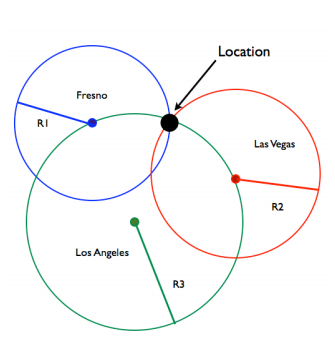
\includegraphics[width=.25\textwidth]{images/Mobile computing/4. Posizione/distanza esatta.PNG}
        \end{center}
        
        \item \textbf{upper bound} della distanza: "la distanza è al più...".
        Molte tecniche forniscono una distanza massima del device da una posizione nota.
        Se ho un solo oggetto so che la posizione sarà all'interno della circonferenza. Se ho due o più oggetti, la X starà nell'intersezione.
        \\ 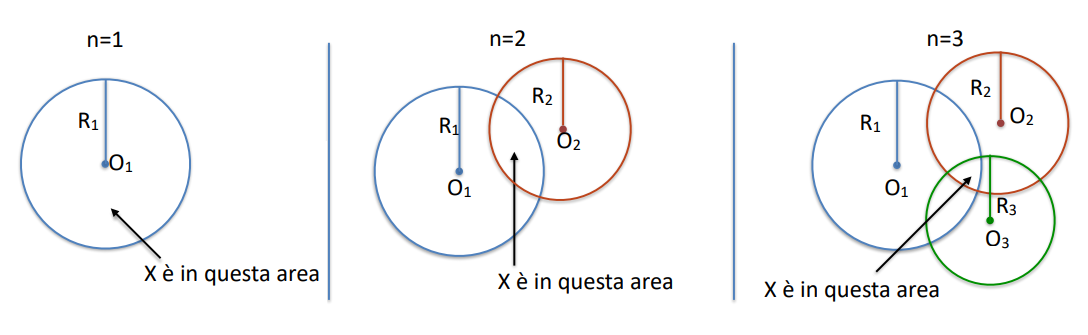
\includegraphics[width=.9\textwidth]{images/Mobile computing/4. Posizione/upper bound.PNG}
        \item \textbf{range di distanza}: "la distanza è compresa tra ...". \\
        \begin{minipage}{.4\textwidth}
           Possiamo definire il problema in modo più generale considerando che per ogni oggetto $O_i$ conosco una distanza minima e massima rispetto ad x
        \end{minipage} 
        \hfill
        \begin{minipage}{.6\textwidth}
            \begin{center}
                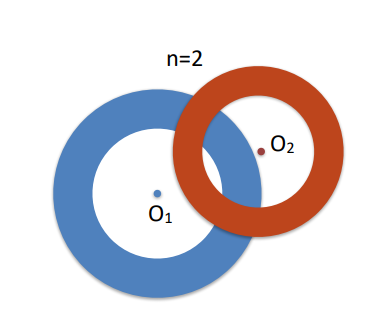
\includegraphics[width=.45\textwidth]{images/Mobile computing/4. Posizione/range di distanza.PNG}
            \end{center}
        \end{minipage}
    \end{itemize}
\end{itemize}

In tutti i casi abbiamo una stima della distanza, ma la stima può essere errata. 
Il sistema di calcolo della posizione deve essere in grado di gestire anche questi casi, ad esempio provando ad identificare la stima errata sulla base delle altre. 
\begin{center}
    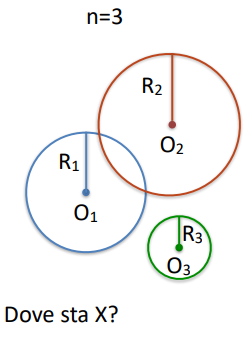
\includegraphics[width=.3\textwidth]{images/Mobile computing/4. Posizione/stima errata.PNG}
\end{center}
In questo esempio posso stimare che la posizione di X sia nell'intersezione tra R1 ed R2 ma nel punto più basso, perché devo anche considerare R3. 

\section{Calcolo della posizione outdoor}
La posizione outdoor si calcola con 3 soluzioni: 
\begin{itemize}
    \item Global Navigation Satellite System (GNSS) 
    \item Rete Cellulare 
    \item WiFi Network based
\end{itemize}
Queste tecniche da sole non funzionano, devono essere combinate con altre tecniche ibride.

\subsection{Global Navigation Satellite System (GNSS) }
Ci sono una serie di satelliti che viene messa in orbita e in ogni istante possiamo sapere la loro posizione.
Hanno a bordo un orologio atomico che gli permette di sapere l'ora in modo preciso.
Mentre i satelliti ruotano, inviano il proprio id insieme all'informazione temporale. 

Il dispositivo mobile riceve l'informazione e riesce a calcolare la distanza da uno o più satelliti. Sfruttando il tempo di propagazione del segnale posso conoscere la distanza dal satellite (la cui posizione può essere calcolata), quindi si usa una tecnica simile alla trilaterazione per calcolare la posizione.

Abbiamo un problema. Il device non ha un orologio atomico, quindi deve essere sincronizzato e richiede di ricevere il segnale da almeno 4 satelliti. Posso calcolare così la mia posizione nello spazio e la mia posizione precisa. 
Possiamo avere anche problemi legati a:
\begin{itemize}
    \item interferenze: in particolare atmosfera (condizioni meteo) e edifici 
    \item posizione dei satelliti potrebbe non essere esattamente quella prevista
\end{itemize}

Ci sono diversi sistemi in uso: 
\begin{itemize}
    \item GPS (USA): è in grado di fornire una posizione maggiore ma per motivi di sicurezza, la precisione sotto ai 3 metri viene usata in ambiti militari
    \item GLONASS (Russia)
    \item Galileo (Europa): fornisce una posizione sotto al metro
\end{itemize}

Ci sono due modi per diminuire i problemi del segnale satellitare:
\begin{itemize}
    \item Differential GPS (D-GPS): è un sistema che permette di correggere (almeno in parte) l'errore dovuto alle interferenze dell'atmosfera e ad una non precisa posizione dei satelliti rispetto a quanto previsto. Consiste nell'avere stazioni terrestri collocate in posizioni note che misurano la potenza del segnale dei satelliti. Un ricevitore in posizione fissa a terra calcola la distanza tra il segnale atteso e quello che effettivamente riceve. Il ricevitore poi comunica questa informazione ai dispositivi mobili che dunque possono compensare l'errore
    \item Assisted GPS (A-GPS): il calcolo iniziale della posizione può essere molto lungo (anche qualche minuto) perché il device deve capire quali satelliti sono in vista. A-GPS risolve questo problema:
    \begin{itemize}
        \item ogni antenna della rete cellulare mantiene un elenco dei satelliti in vista 
        \item quando il device deve usare GPS, richiede, tramite un apposito servizio, quali sono i satelliti in vista all'antenna più vicina. Saranno gli stessi in vista al device (l’antenna non può essere troppo lontana) 
    \end{itemize}
    Questo riduce notevolmente il tempo di calcolo della posizione che in genere è di pochi secondi
\end{itemize}

\subsection{Rete cellulare}
Un altro modo per calcolare la posizione è attraverso la rete cellulare.
Ogni device è connesso ad un'antenna di cui sono note la posizione e l'area della relativa cella. 
Il problema è che l'approssimazione è molto alta e dipende dalla dimensione della cella. 
Una prima soluzione è il protocollo GSM, che prevede l'uso di una tecnica per stimare la distanza tra il device e l'antenna.
Lo scopo all'interno di GSM è quello di evitare collisioni, c'è quindi una tecnica che permette di stimare la distanza tra il device e l'antenna. 

Oltre al protocollo GSM, possiamo sviluppare tecniche per stimare la distanza tra un device mobile e un'antenna dove usiamo il ritardo id propagazione del segnale per stimare la distanza tra un device mobile e un'antenna di rete cellulare. La precisione è nell'ordine di 50-125 metri. 


\subsection{WiFi positioning}
Ci serve conoscere la distanza tra il device e gli Access Point e la posizione di questi. 

Il protocollo 802.11 (protocollo di base alle reti WiFi) prevede che gli access point comunichino il proprio ID, anche ai device che non sono connessi/autenticati a quella rete.
Possiamo sapere quali sono i device che sono nelle vicinanze e la loro relativa potenza del segnale. Minore è la potenza del segnale, significa che sono lontano, maggiore è la potenza del segnale e più sono vicino.

\subsubsection{Problemi}
La potenza del segnale è approssimativamente proporzionale alla distanza perché ci potrebbero essere delle interferenze, infatti se un device e un AP sono vicini, ma c'è qualcosa che crea interferenza, la potenza del segnale sarà bassa.

Un altro problema è che non sappiamo dove sono posizionati gli AP, per questo usiamo un approccio basato su crowdsourcing, un modo di raccogliere i dati dagli utenti che usano il servizio. 
Il crowdsourcing può richiedere o meno un’azione esplicita da parte degli utenti.
Quando l'utente ha il GPS attivo, calcola la propria posizione con una buona precisione e comunica ad un location service (server) la propria posizione e gli access point nelle vicinanze. 
Il location service riceve le informazioni da più utenti e stima la posizione degli access point. 
Quando un utente non ha il GPS attivo: 
\begin{itemize}
    \item invia al location service l'elenco degli AP nelle vicinanze (e la potenza del segnale) 
    \item il location service calcola la posizione dell'utente e gliela comunica
\end{itemize}

Ogni volta che il device vuole calcolare la posizione, guarda quello che ha e lo comunica al location service che risponde con una posizione. 
Questa è una tecnica ibrida perché è basata su due tecnologie, GPS e WiFi.

\textit{Chi calcola la posizione usando il sistema satellitare? Device o server?}
\\ Il device ha l'antenna e può calcolarlo in autonomia. 

Per il calcolo della posizione WiFi non ho in locale la conoscenza delle posizioni degli AP e quindi ho la necessità di comunicare con un location service. 

